%Het eerste hoofdstuk van je thesis.
\chapter{Opdrachtbeschrijving}
\label{chap:Opdrachtbeschrijving}
De opdracht bestaat erin om een line-following robot te maken. Deze robot wijkt enigszins af van de klassieke line-follower aangezien de circuits die wij moeten kunnen afleggen, bestaan uit 2 volle buitenlijnen en een gestreepte middellijn, waardoor we niet zomaar de middellijn kunnen volgen. Deze uitdagingen maken volgalgoritme zeer ingewikkeld en onvoorspelbaar. We kregen op voorhand 3 verschillende circuits die de robot autonoom zou moeten afleggen terwijl hij simultaan andere taken uitvoert zoals snelheden registreren of RFID-tags uitlezen en deze doorsturen. De breedte van de baan is ongeveer twee maal de breedte van de auto. We kregen een basispakket vanwaar we konden vertrekken dewelke bestond uit het chassis van de robot, 2 motoren, een batterij, een Sparkfun motor shield en 2 Arduino Uno's. We hadden ook steeds een 3D-printer ter beschikking om 3D-onderdelen te printen die we nodig hadden om sensoren te bevestigen en dergelijke. Verder kregen we ook nog een budget van 50 euro ter beschikkingvan de school om ons te voorzien van de nodige componenten. De opdracht bestaat zowel uit het bedenken en ontwerpen van de nodige hardware als het schrijven van de nodige software zodat de robot de 3 verschillende circuits autonoom zou kunnen afleggen.
\section{Hardware}
Voor het ontwikkelen van de software konden we beroep doen op een Arduino Uno en een motorshield van Sparkfun, zoals te zien in Figuur ~\ref{fig:ArduMoto}, maar voor de uiteindelijke opdracht moesten we natuurlijk gebruik maken van zelfvervaardigde printplaten (PCB's). Aan de hand van een schema van de Arduino Uno, dat beschikbaar is op het internet, konden we onze eigen PCB ontwerpen waarbij we alle niet-noodzakelijke componenten weglieten en de L298, de chip die verantwoordelijk is voor de motoraansturing, toevoegden. Voor de sensoren, Bluetooth-module en RFID-reader, waren we vrij om te kiezen.




\begin{figure}[H]
\centering
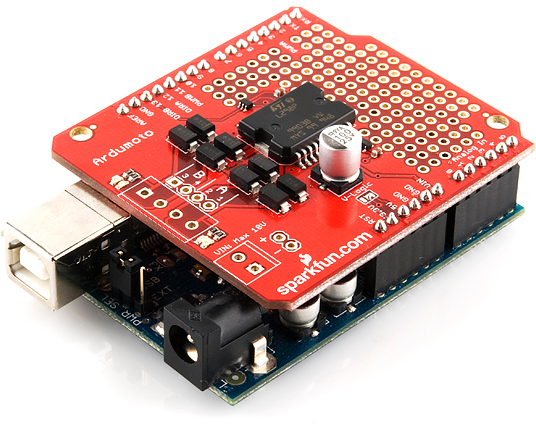
\includegraphics[width=0.75\textwidth]{ArduMoto.png}
\caption{Motorshield gecombineerd met een Arduino. \label{fig:ArduMoto}}
\end{figure}

\section{Software}
Het tweede onderdeel van de opdracht bestaat erin om de Arduino (en later onze eigen PCB) dusdanig te programmeren dat hij autonoom verschillende circuits kan afleggen in een zo kort mogelijke tijd. Er werd ons aangeraden te werken met een PID-regeling om een zo stabiel mogelijke robot te verkrijgen. Tijdens het afleggen van het circuit moet de robotd ata via Bluetooth doorsturen naar de Raspberry Pi.


 



